\chapter{Background and Related Works} In the domain of High-Performancell
Computing (HPC) and data center networks, the coordination of numerous hardware
components is crucial for them to function as a unified system. This
coordination happens through an interconnection network, which serves as the
backbone for communication among these components. Thousands of hardware pieces
collaborate over this interconnection network to ensure smooth operation. The
effectiveness of this interconnect relies on various design choices, such as the
topology used to connect physical components, the routing scheme to select
communication paths, and managing network traffic loads along these paths and
links.  In this chapter, I provide essential background information on topology,
routing and Software Defined Networks (SDN). These fundamental concepts, will give readers the insight into how hardware components interact and how interconnect designs can be optimized for better performance within HPC and data center environments.

\section{Topology} The interconnect network is often represented as a graph, where each node represents a piece of hardware like a server or a switch,
and each line (edge) represents a link between them. Servers are referred to as processing elements, while switches and routers are referred to as forwarding elements. Two nodes directly connected by a link are neighbors. The
number of links a node has is called its nodal degree~\cite{dally2004principles}. The distance
between two nodes is how many links (or hops) it takes to get from one to
the other~\cite{dally2004principles}. The diameter of a network is the longest distance between any two
nodes.  Splitting the network into two equal halves is called a bisection, and
the bandwidth of this split is how much data can flow between the two halves
without slowing down~\cite{dally2004principles}. The bisection bandwidth is the lowest possible bandwidth
among all possible splits. In HPC and data-center networks, low diameter and high bisection bandwidth are essential for performance, whereas a low nodal degree reduces costs and simplifies the design~\cite{li2016low}. To meet these challenges,
different types of topologies are used. In data centers, one of the most
commonly utilized interconnection topologies is the fat-tree. This design has
gained popularity due to its ability to efficiently provide a high throughput
and low latency for communication. For bigger systems, like exascale
supercomputers, the dragonfly topology has been gaining popularity recently.
It's designed to be scalable and cost-effective on a large scale. As technology
evolves, new topologies will likely be developed to meet the demands of future
interconnects.

\subsection{Fat-tree} Fat-tree topology represents a robust architecture for
high-performance computing environments, characterized by its hierarchical
structure and abundant bandwidth allocation~\cite{leiserson1985fat}. In this topology, switches and
compute nodes are organized into a tree like structure, with bandwidth
increasing as one ascends toward the root of the tree. In a typical fat-tree setup, such as the 3-level full bisection bandwidth
fat-tree, switches are classified into three categories: 

\begin{itemize} 
\item \textbf{Core Switches :} These switches reside at the highest layer and serve to interconnect different pods~\cite{al2008scalable}.
\item \textbf{Aggregate Switches :} Positioned between the core and leaf switches, aggregate switches link to the leaf switches within a pod, forming a cohesive unit.
\item \textbf{Leaf Switches :} Located at the bottom layer, leaf switches interface directly with the compute nodes, facilitating communication within the pod.
\end{itemize} 
Figure ~\ref{fig:ftree_ex} shows a example of a three level fat-tree.
\begin{figure}[h!]
  \centering
  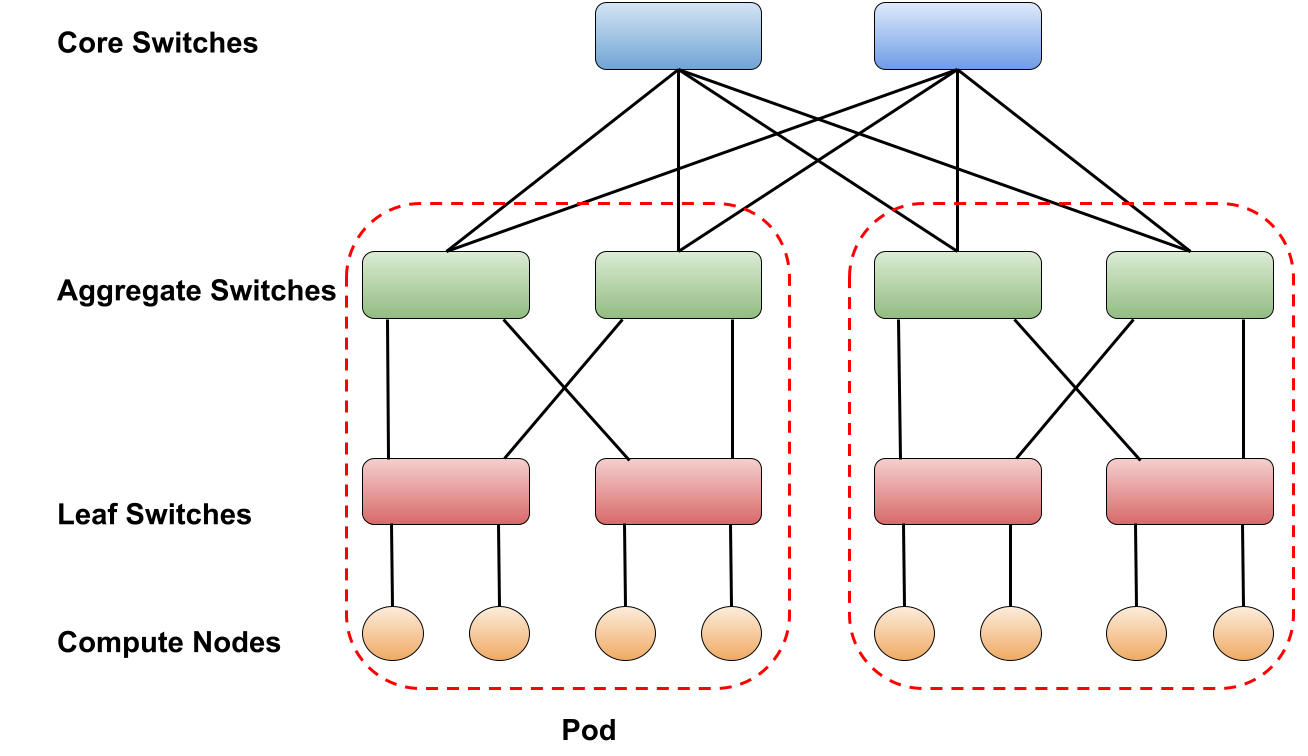
\includegraphics[width=0.8\columnwidth]{./figs/ftree_ex.png}
  \caption{A three level fat-tree with core, aggregate, leaf switch levels and pods.}
  \label{fig:ftree_ex}
\end{figure} 


Nearly every practical fat-tree topology can be expressed through the extended generalised fat-tree (XGFT) notation~\cite{nienaber2014effective}. An XGFT is a parameterised model for fat-tree interconnects defined as
\[
\mathrm{XGFT}\!\bigl(h; m_{1},\ldots,m_{h};\, w_{1},\ldots,w_{h}\bigr),
\]
where h is the height of the tree, a switch at level~$i$ has \(m_{i}\) downward links to children and \(w_{i}\) upward links to parents. Compute nodes attach at level~0, and the total number of nodes is
\[
N \;=\; \prod_{i=1}^{h} m_{i}.
\]

Figure~\ref{fig:fat-treexgft} shows, in four steps, how to build a three-level fat-tree with XGFT notation.  
First, start with a single node, since there no links and the height of the tree is 0, the XGFT notation is $\mathrm{XGFT}(0;\,;\,)$.  
Second, connect four of these nodes with one switch, which is also called leaf switch; this makes
$\mathrm{XGFT}(1;\,4;\,1)$, where every node has one link going up and the leaf switch has four links going down.  
Third, create four copies of that one-level tree and join the leaf switches to two aggregate switches, giving
$\mathrm{XGFT}(2;\,4,4;\,1,2)$, here 4 links go down from each aggregate switch to leaf switches, and two links go up from 
each leaf switch to connect to the aggregate switches.  
Last, connect three of these two-level trees to four core switches to form the three level fat-tree. Since each core switch has 3 downlink and each aggregate switch has 2 uplinks, the XGFT notation is $\mathrm{XGFT}(3;\,4,4,3;\,1,2,2)$. 
\begin{figure}[h!]
  \centering
  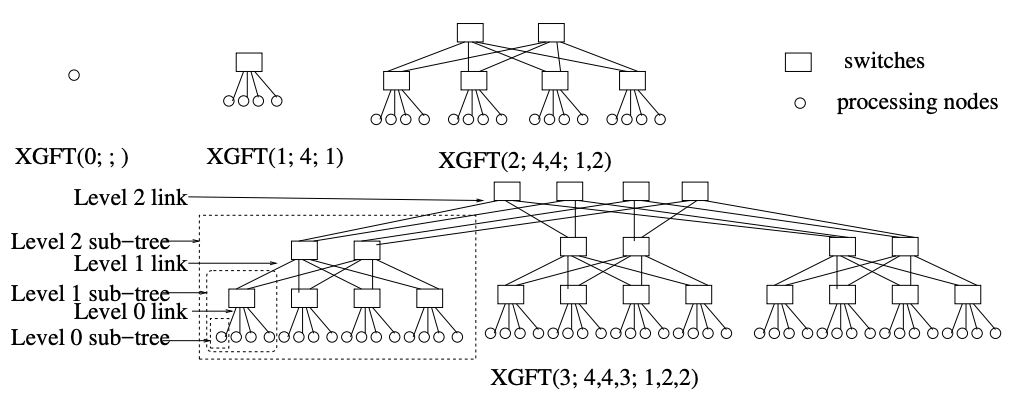
\includegraphics[width=0.8\columnwidth]{./figs/xgft.png}
  \caption{A fat-tree represented in XGFT.}
  \label{fig:fat-treexgft}
\end{figure}

A fat-tree is said to provide full bisection bandwidth when every internal switch offers as many upward links as there are downward links feeding into it~\cite{priceinfiniband}, i.e.,
\[
  w_{i}=m_{\,i-1}\qquad\text{for all }i=1,\dots ,h .
\]
This 1:1 balance of ingress and egress capacity at each switch means packets that arrive from the layer below can be forwarded upward without blocking.  Because each level preserves the available bandwidth, the minimal cut that divides the end hosts into two equal halves of nodes has a combined capacity matches the total injection bandwidth of either half, thereby guaranteeing full bisection throughput.  In a three-level fat-tree, for instance, \(m_{1}=w_{2}\) and \(m_{2}=w_{3}\) uphold this property.

One method used to reduce the cost of building a fat-tree network is
tapering~\cite{Jain:sc2017}. Tapering involves connecting more devices to each switch at the lower
levels of the network. While this may decrease the total
bandwidth available at higher levels, it also reduces the number of switches and
cables needed to connect the same number of devices compared to a full bisection fat-tree.
A tapered fat-tree is obtained by provisioning fewer uplinks than downlinks at one or more switch levels. In XGFT notation a tree is tapered if
\(
  w_{i}<m_{\,i-1}
\)
for at least one \(i\in\{1,\dots ,h\}\).
The tapering ratio is the ratio of number of downlinks to the number of uplinks in a switch at a given level, it determines the extent of uplink reduction~\cite{Jain:sc2017, taffet2019testing}. In a 3-to-1 tapering configuration, for every one uplink from a leaf switch, three downlinks connect to three compute nodes each.
The figure below (Figure~\ref{fig:tapered_ft}) illustrates a tapered fat-tree pod for a 3-level fat-tree with 32 port switches.
\begin{figure}[h]
  \centering
  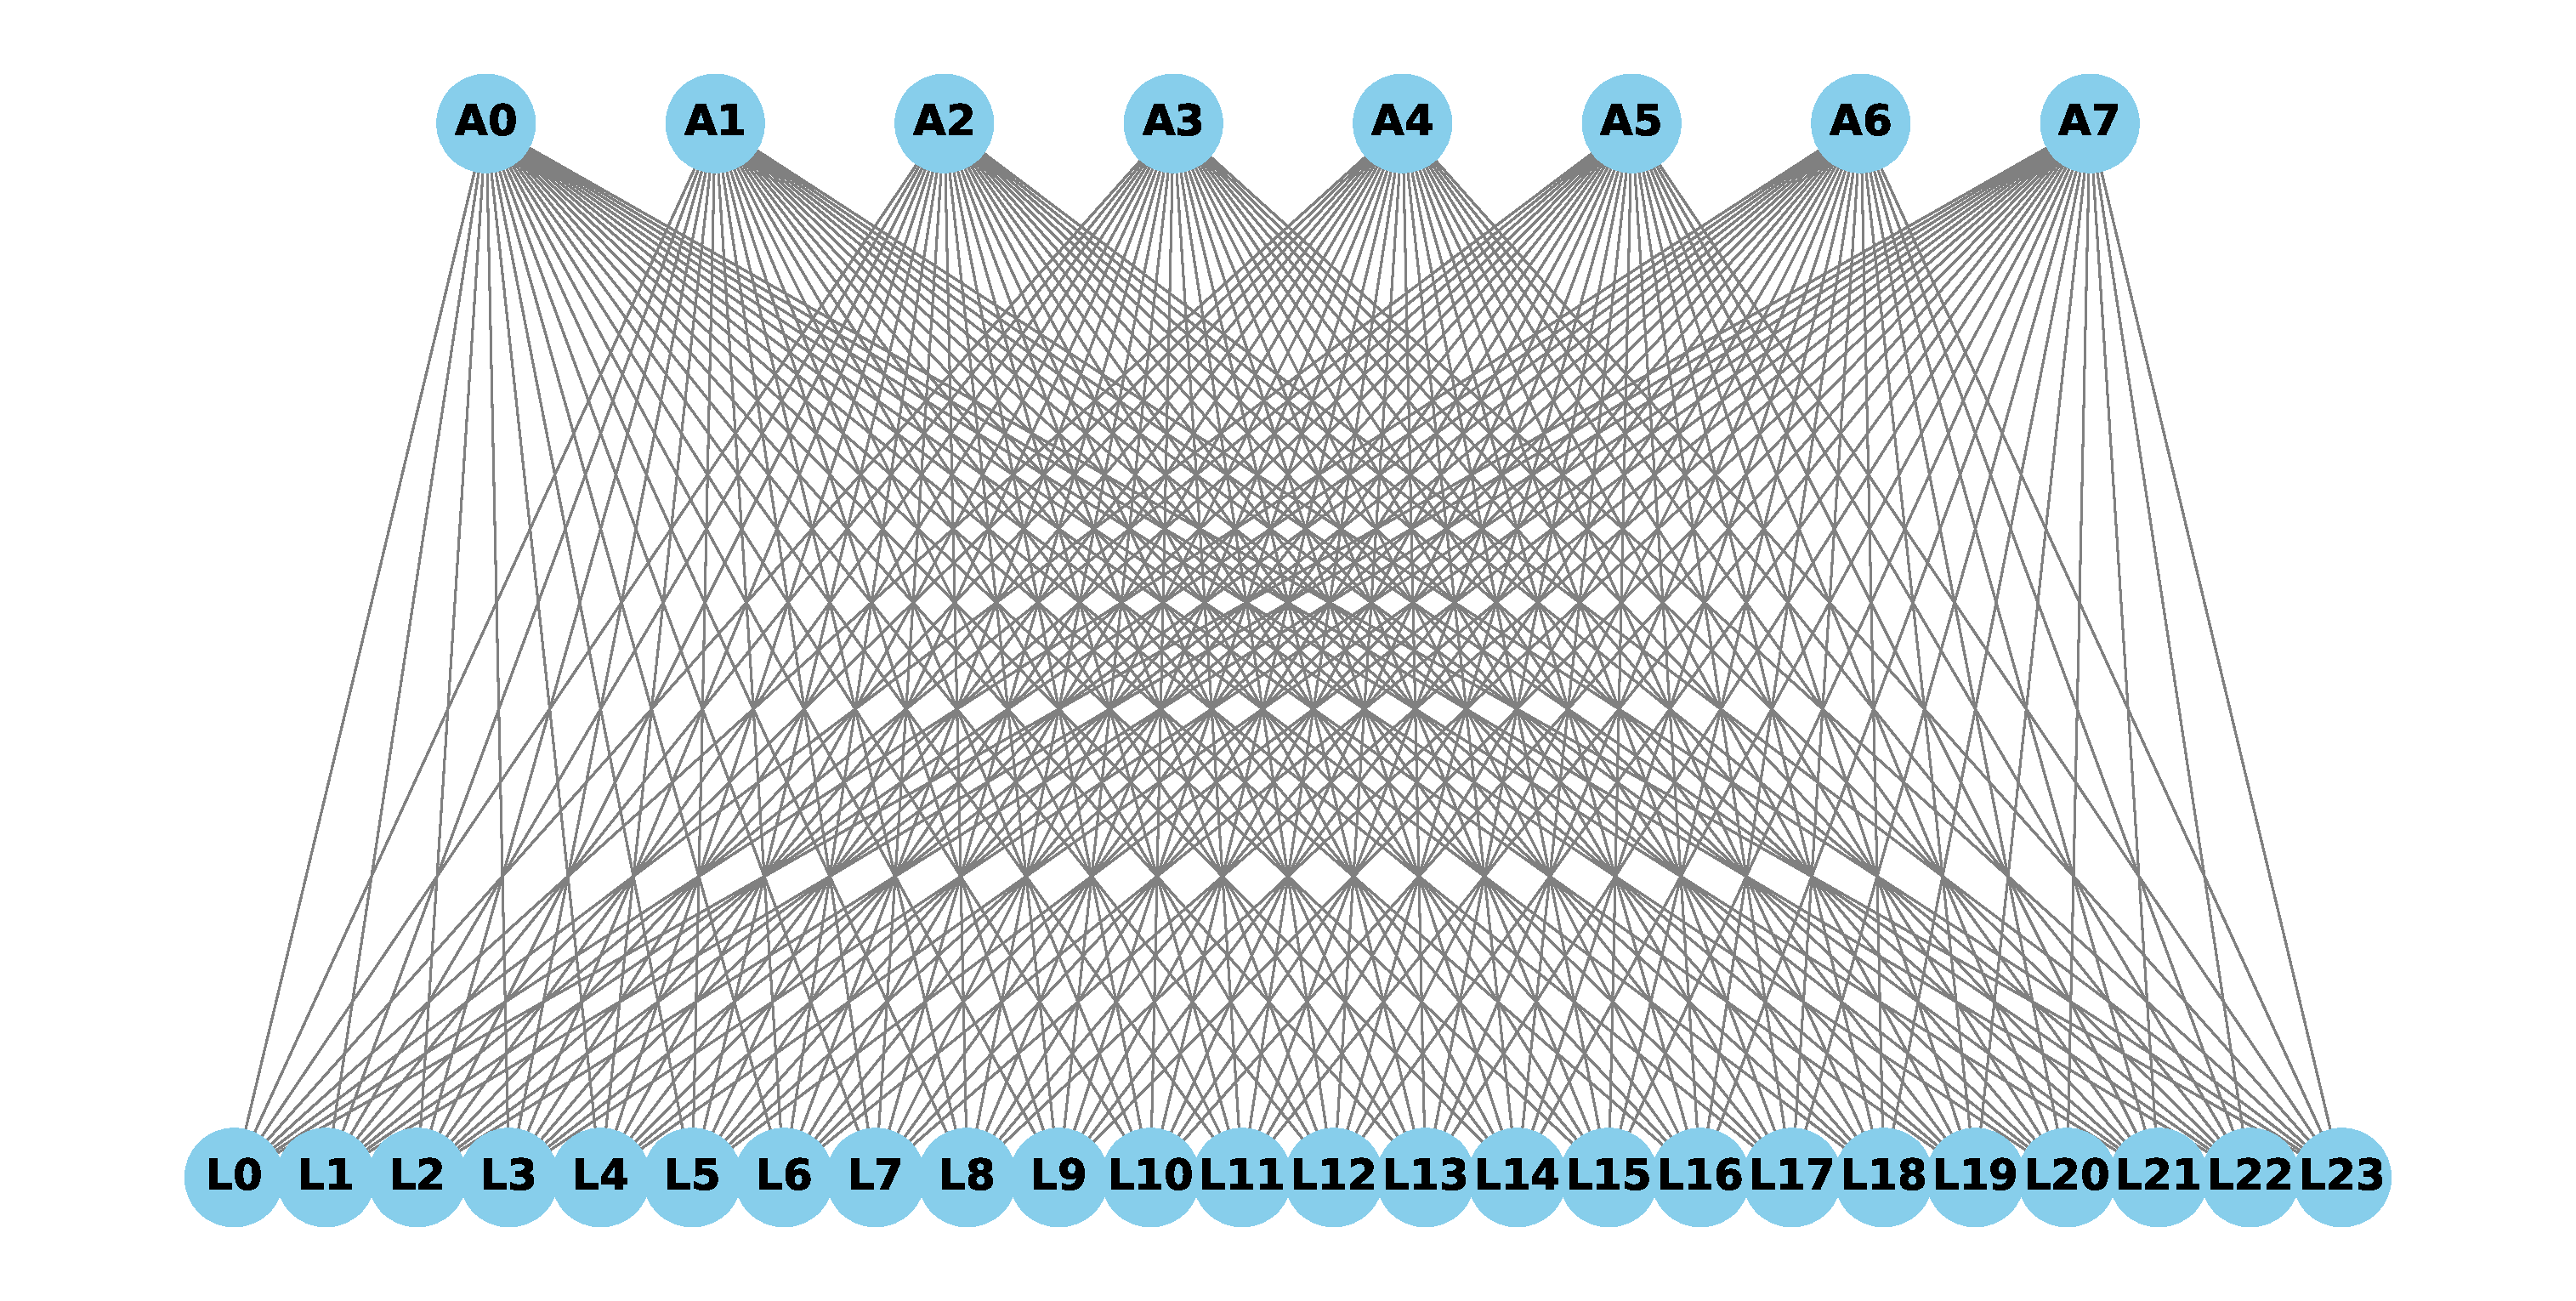
\includegraphics[width=\columnwidth]{./figs_4/tapered_fat_tree_pod.pdf}
  \caption{3-to-1 Tapered Fat-tree pod}
  \label{fig:tapered_ft}
\end{figure}


\subsection{Dragonfly} The dragonfly topology stands out as a cost-effective
solution for building expansive interconnection networks~\cite{kim2008technology}. This design is
characterized by its two-layer structure, exemplified in Figure \ref{fig:dfly}. Initially
proposed by Kim et al.~\cite{kim2008technology}, the dragonfly topology employs a multi-level dense
configuration, primarily leveraging high-radix routers.  In its basic form, a
dragonfly network comprises interconnected routers forming groups, each
resembling a virtual router with a notably high radix [8]. These groups are then
interconnected through an inter-group topology. 
Figure \ref{fig:dfly} illustrates a sample dragonfly network with nine groups, each containing four switches.
There are variations of
dragonfly topology, including canonical dragonfly, hamming dragonfly, and
dragonfly plus, which utilize various intra-group connectivity patterns~\cite{hastings2015comparing}.
However, all implementations of dragonfly topology feature all-to-all
connectivity between groups. 

\begin{figure}[h!]
  \centering
  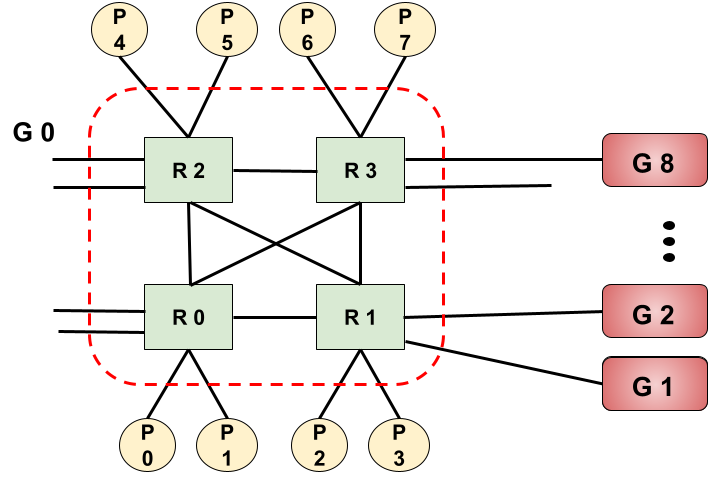
\includegraphics[width=0.8\columnwidth]{figs/dfly1.png}
  \caption{Dragonfly architecture with 9 groups and 4 routers per group}
  \label{fig:dfly}
\end{figure}


Four fundamental parameters characterize the dragonfly topology: the number of compute nodes in each switch (p), the intra-group links per switch (a), the
inter-group links per switch (h), and the total number of groups (g)~\cite{kim2008technology}. 
The dragonfly network comprises of $g \times a$
 routers, and $g \times a \times p$ compute nodes, where g represents the
number of groups, a signifies the intra-group links per switch, and p
denotes the compute nodes per switch. Each group has $a \times h$ global links, with
h representing the inter-group links per switch. Notably, the maximum size
dragonfly configuration is characterized by $g = a \times h + 1$ groups. 
Several prominent supercomputer
architectures, such as the Cray Cascade architecture and the Cray Slingshot
network, have embraced variations of the dragonfly topology~\cite{faanes2012cray, de2020depth}. These
implementations have found their way into current supercomputers like Titan~\cite{titan} and
Trinity~\cite{archer2015trinity}, as well as future exascale computing designs.  In summary, the
dragonfly topology, with its versatile structure and efficient utilization of
high-radix routers, presents a compelling solution for constructing large-scale
interconnection networks, offering both cost-effectiveness and scalability.

\section{Routing}

Routing in determines how data packets, which are units of data transmitted over a network, travel from a source to an destination within a network. Each data packet contains information such as the source address, destination address, and the actual data being transmitted. These packets are sent from a source node to a destination node, with each node being connected to a switch. The source switch connects to the source node, while the destination switch connects to the destination node. It involves mapping network flows to specific paths for data transmission, a process influenced by the network's underlying topology. The efficiency of routing directly impacts the performance of applications in HPC and data center systems, making it a crucial aspect of interconnect modeling.
Routing in interconnect networks can be classified into three broad categories: when the routing decision is taken, how the path is selected, and where the decision is taken~\cite{scheideler2006universal, dally2004principles}. In terms of the timing at which the routing decision is made, there are offline schemes and online schemes; offline schemes establish routes statically during system configuration, whereas online schemes compute routes at runtime to mitigate congestion. In terms of path selection, there are deterministic routing, oblivious routing, and adaptive routing. Deterministic routing assigns a single, immutable path to each source–destination node pair; oblivious routing chooses among multiple paths without considering current network conditions; and adaptive routing uses real-time network indicators such as queue occupancy or link utilisation to select a path from a set of paths. Finally, in terms of the location at which the decision is made, there are source routing and distributed routing. In source routing, the entire path is encoded in the packet header at the source node, whereas in distributed routing each intermediate node along the path makes routing decisions based on local routing tables or forwarding rules.
These routing strategies play a vital role in ensuring efficient data transmission in HPC and data center environments.

\subsection{Routing in Fat-tree}
Routing strategies within fat-tree networks can be categorized as either oblivious or adaptive to network communication traffic. In fat-tree networks, oblivious routing algorithms consistently select the same nearest common ancestor (NCA) for all communication between a given source-destination pair. These routing paths can be pre-computed and stored in forwarding tables or calculated dynamically based on simple formulas using source and destination labels. Two common static oblivious routing schemes in fat-tree networks are source-mod-k (S-mod-k) and destination-mod-k (D-mod-k). In S-mod-k at each upward hop, the switch selects port
$(s \bmod k)$, where~$s$ is the numeric identifier of the source node and k is the number of uplinks from the current switch. Simillarly, in D-mod-k, the switch selects port
$(d \bmod k)$, where~$d$ is the numeric identifier of the destination node~\cite{rodriguez2009oblivious, mahapatra2012limited}. In both these routing, after the packet reaches the NCA, it travels downward along the unique path to the destination node. Although, these routing algorithms are widely used in many HPC systems as the default static routing algorithm, they may exhibit poor performance for both average and worst-case permutation traffic patterns. 

Adaptive routing dynamically select paths based on the current network state, such as link congestion or available bandwidth, to optimize performance in real-time. During the upward direction toward the nearest common ancestor (NCA) for both the source and destination routers, adaptive routing algorithms prioritize forwarding packets to the least congested port available~\cite{gomez2007deterministic}. This approach helps to alleviate congestion and optimize the utilization of network resources by steering traffic along paths with ample capacity. Once the packet reaches the NCA, which acts as the central router for the source-destination pair, it is then directed along a unique downward path toward the destination router. By dynamically adapting routing paths based on real-time network conditions, adaptive routing enhances the efficiency and performance of fat-tree networks. Routing decisions in fat-tree networks typically focus on determining the upward paths to carry traffic for each source-destination pair.

\subsection{Routing in Dragonfly}
In a dragonfly topology, the source node belongs to the source group, and the destination node belongs to the destination group. Traffic packets between these nodes can travel along either a minimal or a non-minimal path. Broadly speaking, the dragonfly network has three popular routing schemes.

The minimal routing scheme (MIN) proposed by Kim \emph{et al.}~\cite{kim2008technology}
always forwards a packet along the shortest path between a source router~$R_s$ and a destination
router~$R_d$ in a dragonfly topology. If $R_s$ and $R_d$ lie in the same group or both of them are connected by a global link, thepath is a single hop, if one of the router is connected to the global link which goes to the other's group then it is a two-hop path, the packet never travels more than one global link. 
A minimal path comprises no more than three hops:

\begin{enumerate}
  \item a local hop inside the source group to a gateway router~$R_a$ that owns a global
        link to the destination group;
  \item a single global hop from $R_a$ to a gateway router~$R_b$ in the destination group;
  \item a local hop from $R_b$ to the destination router~$R_d$.
\end{enumerate}

Its deterministic nature, however, makes it vulnerable to adversarial permutations such
as the shift pattern, in which every router of a source group simultaneously send to the same
destination group as such the global link between the two groups is shared by all routers
to send its data, and it becomes a bottleneck.


Valiant Load-Balanced Routing (VLB)~\cite{kim2008technology, kaplan2017unveiling}, sends each packet through a randomly chosen intermediate router in an intermidiate group before it reaches its destination. This detour spreads traffic evenly across the
fabric and removes congestion that can happen when many packets tries to use the same global link to reach their destination. A packet routed in VLB path can traverse up to two global links and no more than five hops:
\begin{enumerate}
  \item a local hop inside the source group from the source router \(R_s\) to a
        gateway router \(R_a\) that has a global link to the intermediate group;
  \item a global hop from \(R_a\) to a gateway router \(R_b\) in the
        intermediate group;
  \item a local hop within the intermediate group from \(R_b\) to another
        gateway router \(R_c\) that owns a global link to the destination group;
  \item a second global hop from \(R_c\) to a gateway router \(R_t\) in the
        destination group; and
  \item a final local hop from \(R_t\) to the destination router \(R_d\).
\end{enumerate}
By randomising the choice of the intermediate group, VLB balance the network load in adversarial
traffic patterns, at the cost of the extra distance introduced by the detour. 

Universal Globally-Adaptive Load-balancing (UGAL) is an adaptive routing algorithm that dynamically chooses, for every packet,
between a MIN path and a VLB path~\cite{kim2008technology}. It monitors the amount of data packets queued up or waiting to be transmitted at the source router. By assessing the level of queue occupancy, it can infer the current state of congestion within the network. If the queue occupancy is high, there can be congestion, and it may opt for routing strategies that help alleviate congestion, such as selecting VLB paths to distribute traffic more evenly across available links. 

Two practical variants UGAL are:
\emph{UGAL-G} which assumes perfect, system-wide knowledge of queue occupancies and is
used mainly as an upper-bound benchmark.
\emph{UGAL-L}, which relies only on local queue occupancy information at the the source
router.  
Let $q_m$ and $q_{nm}$ denote the output-queue occupancies of the first link on
the minimal and non-minimal paths, and let $H_m$ and $H_{nm}$ be the respective
hop counts ($3$ and $5$ in a dragonfly).  
UGAL-L approximates the latency of each path as the product of these two
quantities and introduces a bias~$b$ that tilts the decision toward MIN path or
the VLB path.  
A packet is routed minimally only if
\[
  q_m \times H_m \;\le\; q_{nm} \times H_{nm} + b,
\]
otherwise it is routed non-minimally.  



\section{HPC Applications}
\label{sec:exp}
In high-performance computing, workloads comprise real applications, which address substantive scientific, engineering, finance and other real-world problems, and proxy applications, which imitate the computational and communication characteristics of real applications in a reduced form. Moreover, system architects employ synthetic traffic patterns, which are artificially constructed sequence of message transfers, to evaluate performance under carefully controlled conditions.
Many HPC applications share a common iterative structure, each iteration entails a sequence of computational tasks executed in parallel, followed by communication and synchronization steps. These iterations form the backbone of many HPC workflows, where complex computations are distributed across vast computational resources. As data flows through the system, results are exchanged, aggregated, and synchronized to drive iterative refinement and convergence.

In my work I have chosen a set of benchmarks which is represents the diverse HPC workloads along with some synthetic traffic, to ensure that the performance evaluation of my algorithms is comprehensive and applicable across a wide array of HPC scenarios.
The following is a brief description of the applications I used in this work:

\begin{itemize}
\item \textbf{Random permutation}: A synthetic traffic where each node sends a message to another randomly chosen node. The source destination pair is unique across the whole permutation.
\item \textbf{Stencil3d}: MPI benchmark with 6-point near-neighbor communication in a 3D virtual process grid.
\item \textbf{Stencil4d}: MPI benchmark with 8-point near-neighbor communication in a 4D virtual process grid.
\item \textbf{Random mixed}: A synthetic traffic which is composed of two different random permutation.
\item \textbf{Stencil mixed}: MPI benchmark which is composed of stencil3d kernel followed by stencil4 kernel together.
\item \textbf{Random permutation third}: A synthetic traffic where only a third of the flows in random permutation is used. 
\item \textbf{Subcomm3d}: MPI benchmark with all-to-all communication within subsets of processes in a 3D virtual process grid.
\item \textbf{Kripke}: 3D $S^n$ deterministic particle transport code, which runs an MPI-based parallel sweep algorithm~\cite{kripke}. 
\item \textbf{Laghos}: Proxy application that solves time-dependent Euler equations with MPI-based domain decomposition~\cite{laghos}.
\item \textbf{AMG}:  Parallel algebraic multigrid solver~\cite{amg}.
\item \textbf{SW4lite}: Proxy application for SW4~\cite{sjogreen2018sw4}, a 3D seismic modeling code.
\item \textbf{Lammps}: LAMMPS is an acronym for Large-scale Atomic/Molecular Massively Parallel Simulator, it solves equations of motion for a collection of interacting particles. It partitions the simulation domain into small sub-domains to solve a problem~\cite{thompson2022lammps}.
\item \textbf{Nekbone}: Solves 3D Poisson problem in rectangular geometry. The key MPI operations are matrix-matrix multiplication, inner products, nearest neighbor communicaton, MPI\_Allreduce~\cite{gong2016nekbone}.
\item \textbf{MILC}: Performs four dimensional SU(3) lattice gauge theory, mainly through near-neighbour communication and MPI\_Allreduce~\cite{gottlieb2001benchmarking}.
\end{itemize}

While evaluating these diverse HPC benchmarks, it is essential to understand the communication characteristics that fundamentally influence their performance and scalability. HPC applications typically exhibit two primary communication characteristics: regular (static) and irregular (dynamic and dynamically analyzable) communication patterns. Recognizing these patterns allows for more precise optimization of network resources, thereby enhancing overall efficiency and performance.

\begin{itemize}
\item \textbf{Regular communication:} Regular communication in HPC applications involves predictable and repetitive data exchanges that are determined before the execution of the application. This type of communication includes static communication patterns where the source and destination nodes, as well as the message sizes, are all known during compile time. Figure ~\ref{code.stencil} displays an MPI code segment of Stencil4d, a representative HPC kernel.
This kernel performs nearest neighbor communication: each process communicates with its 8 neighbors (front/back, top/bottom, left/right, and north/- south) in the 4-dimension domain with 8 MPI Isends and 8 MPI Irecvs. The figure only shows one MPI Isend and one MPI Irecv since the others are similar. The communicator MPI COMM WORLD remains fixed during the execution, and the source and destination, in this case process north of the present node, as well as the message size are known before the application executes. Hence, these communications are static. 
Most communications in HPC applications are static, allowing for more straightforward optimization and improved overall performance by leveraging the predictability of these communication patterns.

\item \textbf{Irregular communication:} 
In HPC applications, communication is irregular when the data-transfer pattern cannot be determined prior to program execution. Most irregular communications are dynamic or dynamically analyzable.
In dynamically analyzable communication, the source and destination nodes
, as well as message sizes, can be determined at runtime but not 
during compile time. For dynamic communication, these parameters cannot be determined 
until after the communication has occured. Figure ~\ref{code.laghos} displays an MPI code segment of the primary solver function for Laghos. In Laghos, a new communicator is established each time the function is called, and communications are performed in that communicator as can be seen in Line 3 of the figure. The communication information for this application is unknown until the communication is performed and the communications are thus dynamic.

\end{itemize}

\begin{figure}[H]
\begin{lstlisting}[breaklines, language=C++, frame=single, tabsize=4, basicstyle=\ttfamily]
for (int i = 0; i < MAX_ITER; i++) {
        MPI_Isend(sendn, 100000000, MPI_CHAR, north, 9, MPI_COMM_WORLD, &reqs[0]
);
        ...
        MPI_Irecv(recvn, 100000000, MPI_CHAR, north, 9, MPI_COMM_WORLD, &reqs[8]
);
        ...
        MPI_Waitall(16, req status);
}
\end{lstlisting}
\caption{Stencil4d code snippet}
\label{code.stencil}
\end{figure}

\begin{figure}[H]
\begin{lstlisting}[breaklines, language=C++, frame=single, tabsize=4, basicstyle=\ttfamily]
LagrangianHydroOperator (...){
        ...
        ParMesh *pm = H1FESpace.GetParMesh();
        MPI_Allreduce(&loc_area, &glob_area, 1, MPI_DOUBLE, MPI_SUM, pm->GetComm
());
        ...
}
\end{lstlisting}
\caption{Laghos code snippet}
\label{code.laghos}
\end{figure}

\section{Software Defined Network}
Software Defined Network(SDN) is a modern networking scheme where, the organization of network functionality is often conceptualized into three distinct layers: the data plane, the control plane, and the management plane~\cite{kreutz2014software}. Each layer serves a critical role in facilitating the efficient operation and management of the network infrastructure. Figure ~\ref{fig:sdn_abs} shows the three planes in the realm of SDN abstraction.

\begin{figure}[h!]
  \centering
  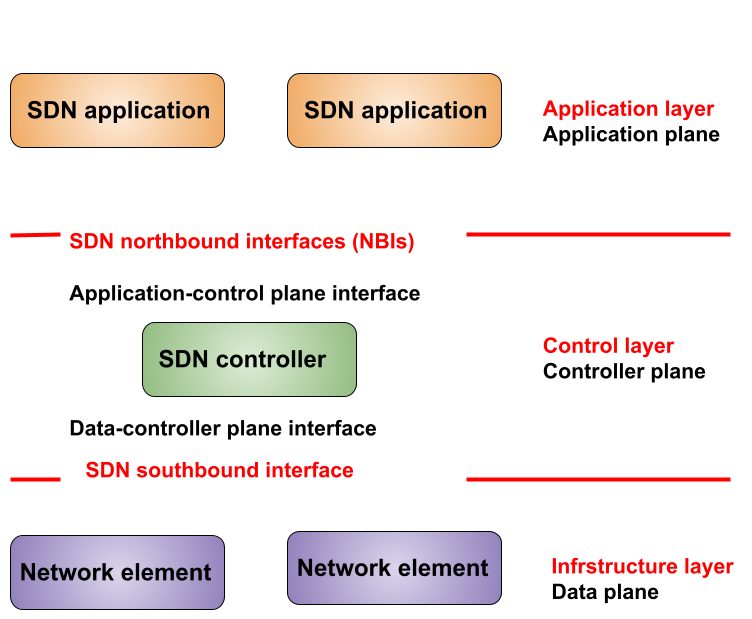
\includegraphics[width=0.8\columnwidth]{figs/sdn_abstraction.png}
  \caption{SDN abstraction }
  \label{fig:sdn_abs}
\end{figure}


\begin{itemize}
\item  \textbf{Data Plane:} The data plane, also known as the forwarding plane, is responsible for the actual transmission of data packets within the network~\cite{tr2016sdn}. It consists of networking devices such as routers, switches, and other forwarding elements. These devices receive incoming packets and make forwarding decisions based on predetermined rules or protocols. The primary function of the data plane is to ensure that data packets are correctly routed to their intended destinations across the network.
\item  \textbf{Control Plane:} The control plane is tasked with managing the forwarding and routing mechanisms within the network~\cite{tr2016sdn}. It determines how data packets should be forwarded based on factors such as network topology, traffic conditions, and routing policies. Traditionally, the control plane functions are embedded within the networking devices themselves, leading to a tightly coupled architecture where control and data planes operate in conjunction with each other. This tightly integrated approach has been essential for ensuring network resilience and stability, particularly in large-scale distributed networks such as the Internet.
\item \textbf{Management Plane:} The management plane oversees the overall management and configuration of the network infrastructure~\cite{tr2016sdn}. It is responsible for tasks such as network monitoring, configuration management, performance optimization, and security policy enforcement. The management plane provides administrators with the tools and interfaces necessary to manage and control various aspects of the network, ensuring its reliability, security, and efficiency.
\end{itemize}

While the traditional networking architecture with tightly coupled control and data planes has been successful in ensuring network resilience, it also poses several limitations. One of the primary challenges is the complexity and rigidity of the architecture, which makes it difficult to introduce innovations and adapt to changing network requirements. Additionally, the decentralized nature of the control plane makes it challenging to achieve a holistic view of the network, hindering effective management and optimization.
To address these limitations and enable greater flexibility and agility in network management, the concept of Software-Defined Networking (SDN) has emerged as a promising approach. SDN decouples the control plane from the data plane, allowing for centralized management and programmability of the network. In an SDN architecture, the control logic is moved to a centralized entity known as the controller or Network Operating System (NOS), which maintains a global view of the network and is responsible for configuring forwarding policies.

The key components of an SDN architecture include the following:

\begin{itemize}

\item \textbf{Decoupled Data and Control Planes:} By separating the control logic from the underlying networking devices, SDN enables greater flexibility, scalability, and agility in network management. It allows administrators to dynamically adjust network behavior in response to changing traffic patterns and application requirements, leading to improved performance and resource utilization~\cite{tr2016sdn, kreutz2014software}.

\item \textbf{Centralized Controller:} The centralized controller serves as the brain of the SDN architecture, maintaining a global view of the network and orchestrating the forwarding policies for all connected devices. The controller communicates with the networking devices via standardized protocols such as OpenFlow, providing a centralized point of control for the entire network~\cite{tr2016sdn, kreutz2014software}.

\item \textbf{Programmable Network Behavior:} One of the key advantages of SDN is its programmability, which enables administrators to implement innovative networking services and applications through software applications running on top of the SDN controller. This programmability allows for the dynamic creation and deployment of network policies, enabling administrators to tailor the network behavior to specific application requirements and business needs~\cite{tr2016sdn, kreutz2014software}.

\end{itemize}




In recent years, SDN has gained widespread acceptance and adoption in both industry and research communities. Its flexibility and programmability have led to a wide range of applications across various domains, including data centers, telecommunications, and cloud computing~\cite{alalmaei2020sdn, faizian2017comparative}. 
One area of particular interest is the application of SDN in high-performance computing (HPC) environments. HPC systems often require fast and efficient communication between compute nodes to handle large-scale scientific computations and data-intensive workloads. By leveraging SDN, researchers aim to optimize routing and topologies in HPC environments, improving communication efficiency and resource utilization.

\begin{figure}[h!]
  \centering
  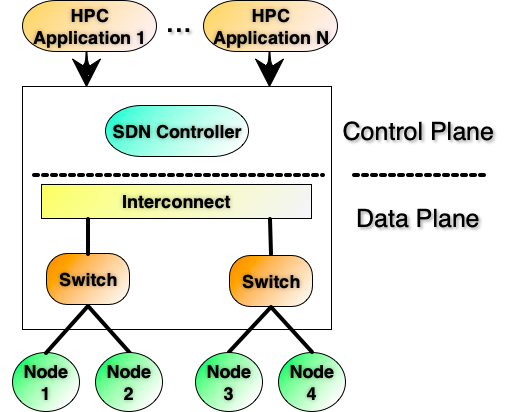
\includegraphics[width=0.8\columnwidth]{./figs/Fig1.png}
  \caption{High-level overview of the SDN-based HPC System}
  \label{fig:sdn_hpc}
\end{figure}

The structure of an SDN based HPC System (SHS) is depicted in Figure~\ref{fig:sdn_hpc}.
The SDN switches perform a simple data plane functionality: packet forwarding. The
control plane is performed by the logically centralized
SDN controller (sometimes called the network operating system), which controls
the SDN switches through an interface~\cite{benzekki2016software}.
The SDN controller provides another layer of network abstraction upon which SDN
applications can be built. When running HPC applications in an SDN based HPC system,
the applications run on the compute nodes connected to the SDN switches,
the applications use the services provided by the SDN controller to perform
communications.




\clearpage
\section{Related Works}
In my dissertation, I focusing on two areas, optimizing hardware parameters for GPU-based HPC platforms 
and incorporating Software Defined Networking (SDN) techniques to improve HPC application performance.

In the first section, I explore the optimization of hardware parameters 
for next-generation GPU-based HPC platforms. Inspired by Jain et al.'s work on fat-tree configurations~\cite{jain2017predicting} 
and studies on dragonfly and jellyfish topologies by Rahman et al.~\cite{rahman2019topology} and Zaid et al.~\cite{alzaid2021multi}, I investigate how different hardware parameters affect network performance through system wide simulation.
Simulations are crucial for evaluating HPC network performance. 
Previous research has utilized simulation tools like TraceR-CODES to analyze various system configurations. 
Jain and Bhatele, for example, used this simulator for detailed analyses 
of different systems, focusing on scalable topologies such as dragonfly, express mesh, and fat-tree~\cite{bhatele2019analyzing}. 
These studies examined the performance of these topologies under different conditions, 
considering factors like the number of nodes, routers, and links, 
which are vital for understanding system costs and performance.
They studied multi-job workloads with diverse communication characteristics 
to assess how link bandwidth, the number of rails, planes, and tapering 
influence system efficiency~\cite{jain2017predicting}. 
My research looks at the impact of varying the number of GPUs per node, 
network link bandwidth, and NIC scheduling policies within 
fat-tree and dragonfly topologies. 
This aims to address how to strike a balance between computation 
and communication capacities by changing the hardware parameters
as HPC systems evolve towards fewer, more powerful nodes.

In the second section, I analyze the integration of SDN techniques in HPC environments.
My work evaluates how network flow classification, phase identification, and SDN-based routing compare with the traditional routing used in fat-tree topologies; it also tries to adapt these techniques for tapered fat-trees, aiming to determine whether incorporating SDN techniques helps run HPC applications efficiently on an HPC system.
Although SDN is successful in other domains, it has not been fully explored in HPC. 
Studies by Faizian et al. have looked at SDN and adaptive routing in 
dragonfly topologies, providing a foundation for my work~\cite{faizian2017comparative}.
Since the introduction of SDN and OpenFlow~\cite{openflow}, the technology has gained acceptance in 
industry and academia. Extensive research has explored SDN capabilities in the HPC domain. 
Arap investigated techniques for efficient MPI collective communications using SDN~\cite{arap2014software}, 
while Takahashi evaluated the performance of the MPI\_Allreduce operation on an SDN cluster~\cite{takahashi2014performance}. 
Additionally, MPI\_Reduce operations on SDN clusters have been developed, 
and efforts are underway to build new MPI libraries that 
take advantage of SDN capabilities. These studies show the potential of SDN to 
improve communication efficiency in HPC environments~\cite{munkhdorj2015design, takahashi2015concept}.

In summary, my research optimizes HPC platforms by bridging the gap between 
computational capacity and communication efficiency and integrating advanced networking paradigms like SDN. 
